\clearpage
\section{Forschungsteil}
\label{sec:work}

% Im Grunde genommen sollte alles in diesem Abschnitt noch einmal umgeschrieben werden, das ist im Moment noch etwas chaotisch.
% Einleitung

Um die Frage zu beantworten, ob es bestimmte Hänge zu einem Paradigma gibt, muss zuerst untersucht werden, wie die Paradigmen mit den Lerntypen zusammenhängen.
Hierbei wird betrachtet, welche Lerntypen Vorteile beim Lernen der Computational Thinking (CT) Aspekte haben könnten.
Außerdem wird geprüft, welche Empfehlungen für die Lerntypen laut Felder und Silvermann mit den Ausrichtungen der Paradigmen zusammenhängen können. Es wird speziell Objektorientierung (OO) als häufigstes Paradigma in Einführungskursen, und funktionale Programmierung (FP) als Fokuspunkt der Arbeit betrachtet.

% Disclaimer
Es werden hierbei vermehrt Annahmen zu den Vorlieben der Lerntypen gemacht, aufgrund der Empfehlungen von Felder und Silvermann im Relation zu den Merkmalen der Paradigma. Aufgrund der zeitlichen Beschränkung der Arbeit können diese Annahmen nicht empirisch überprüft werden.

\subsection{Lerntypen im Zusammenhang mit Computational Thinking}
Programmierkenntnisse zu erlernen bedeutet nicht nur Code zu schreiben, sondern auch CT Kompetenzen zu erwerben.
Nicht jede Lerntypen Dimension zeigt Vor- oder Nachteile beim Lernen der CT Aspekte, allerdings lassen sich einige klare Zusammenhänge herausstellen.

\subsubsection{Auditiv & Visuell}
Visuelle Lerntypen können einen Vorteil beim Erlernen des Konzeptes der Abstraktion haben. Grafische Darstellung ist eine beliebte Art der Darstellung, um Abstraktion in der OO Programmierung zu erklären. Beispielsweise werden Klassen in eigenen Boxen mit ihren Funktionen und Eigenschaften gezeigt, und mit Pfeilen die Verbindungen der verschiedenen Objekte.
Allerdings lässt sich auch notieren, dass auditive Lerntypen generell einen Vorteil in herkömmlichen Vorlesungen haben, da diese meist mit einem frontalen Input gehalten werden. Welche Lerntypen hier einen Vorteil haben, hängt von daher eher davon ab, zu welchen Darstellungsformen sich der Dozent letztenlich entscheidet. % QUELLEN

\subsubsection{Reflektiv & Aktiv}
In der reflektiven aktiven Lerntypendimension lässt sich ein eindeutiger Hang in Hinsicht auf die Kompetenz des Debugging erkennen. Reflektive Lerntypen sind eher dazu veranlagt, ihre Lösungen zu analysieren, und gegebenenfalls zu überarbeiten. Aktive Lerntypen sind als eher risikobereit dargestellt, was vermuten lässt, dass diese dem Debugging weniger Achtung schenken, und eher darauf setzen, schnell viele Lösungen auszuprobieren.

\subsubsection{Sensorisch & Intuitiv}
Beim Aspekt der Abstraktion kann der intuitive Typ einen expliziten Vorteil haben. Intuitive Lerntypen haben von Grund aus einen Hang zum abstrakten Denken, während sensorische Typen sich eher auf etablierte Methoden und Fakten verlassen. Dieser Aspekt wird auch explizit von Felder und Silvermann genannt \cite{felderhandout}. 
Auch im Algorithmischen Denken hat der intuitive Typ durch seine Veranlagung zur Innovation und Abstraktion einen Vorteil. Es wird diesem Typen höchstwahrscheinlich leichter fallen, Probleme neu aufzuarbeiten und abstrakte Lösungen zu finden.

\subsubsection{Sequentiell & Global}
In dieser Lerndimension lässt sich ein Vorteil für sequentielle Lerntypen im Aspekt der Dekomposition erkennen. Das Herunterbrechen auf Teilprobleme ist nicht nur ein wichtiger CT Aspekt, sondern auch eine Veranlagung des sequentiellen Lerntypen, der es sowieso vorzieht, Probleme in einem "Step by Step" Ansatz anzugehen. Der globale Lerntyp könnte hierbei eher Schwierigkeiten haben, da für diese Typen die erfolgreiche Dekomposition zunächst ein weitreichendes Verständnis des Problemes vorraussetzt, welches möglicherweise zeitaufwendiger ist, als für den sequentiellen Typen.

\subsection{Lerntypen in Zusammenhang mit Programmierparadigmen}
Auch bei den Lerntypen des Felder Silvermann Modelles lassen sich teilweise Hänge zu einem bestimmten Paradigma erkennen.

\subsubsection{Auditiv & Visuell}
Hinsichtlich der Unterscheidung zwischen visuellen und auditiven Typen lässt sich beidseitig argumentieren. Beim Erlernen von Objektorientierten Konzepten wie Vererbung bieten sich visuelle Darstellungen wie Graphen an. Allerdings können visuelle Typen auch einfacher mathematische Konzepte auf die Philosophien der funktionalen Programmierung übertragen, und die Zusammenhänge besser verstehen.
Andererseits werden die meisten Vorlesungen in einem Stil gehalten, der auditive Lerner bevorzugt. Da die meisten Personen beide Lernstile beherrschen, kann hier keine definitive Aussage zu den Vor- und Nachteilen der Lerntypen gemacht werden.

\subsubsection{Reflektiv & Aktiv}
In der aktiven und reflektiven Dimension lässt sich in beiden betrachteten Paradigmen ein Vorteil für den reflektiven Typen erkennen. Die praktische Umsetzung von Programmierkenntnissen erfolgen meistens in Einzelarbeit, und erfordern eine stetige Reflektion des Lerners.
Das Erlernen von Programmierkenntnissen könnte theoretisch auch in Gruppenarbeiten erfolgen, allerdings werden die meisten Vorlesungsstile reflektiven Typen einen Vorteil bieten. % Schon sehr spekulativ

\subsubsection{Sensorisch & Intuitiv}
In der sensorisch intuitiven Lerntypendimension lassen sich im Gegensatz zu den anderen Dimensionen klare Hänge zu den Paradigmen erkennen.
Sensorische Typen werden vermutlich OO Programmierung vorziehen, da sie die Objekte im Code an echten Problemen modellieren können. Sie können einen direkten und einfach verständlichen Bezug zur echten Welt aufbauen.
Intuitive Typen hingegen sind besser darin, Abstraktion anzuwenden, und werden daher eher FP bevorzugen. Sie können aufgrund ihres Hanges zu Innovation und Verständnis von abstrakteren Konzepten ohne direkten Bezug zur echten Welt schneller Konzepte der FP verstehen und umsetzen. Die deklarativen Vorgehen der FP werden intuitiven Lerntypen ebenfalls einen Vorteil gegenüber OO Programmierung bieten.

\subsubsection{Sequentiell & Global}
Auch in der sequentiell globalen Dimension lassen sich klare Zusammenhänge zu den Paradigmen erkennen. Globale Lerntypen werden es höchstwahrscheinlich vorziehen, zunächst über eine OO Klasse als großes und ganzes nachzudenken, bevor sie sich mit der Implementierung von Details beschäftigen. Um eine sinnvolle Hierarchie zur Komposition der verschiedenen Klassen zu entwerfen, muss grundlegend ein globaleres Verständnis der Problemes vorhanden sein.
Sequentielle Typen hingegen werden eher FP bevorzugen, da das Paradigma das Herunterbrechen von Problemen in Teilschritte von Grund auf vorsieht. Die Probleme werden in Teilfunktionen behandelt, und erst zum Schluss ergibt sich der Zusammenhang zu einem Programm. Es muss nicht direkt ein globales Verständnis der Lösung vorhanden sein, sondern die Lösung setzt sich eher aus den Teilproblemen zusammen.

\subsection{Vorteile und Nachteile der Lerntypen in den Bereichen}
Zusammengefasst lassen sich also definitiv gewisse Vorteile mancher Lerntypen erkennen. Wie betrachten in diesem Fall die CT und Paradigma Dimensionen seperat.

\begin{figure}[h!]
    \centering
    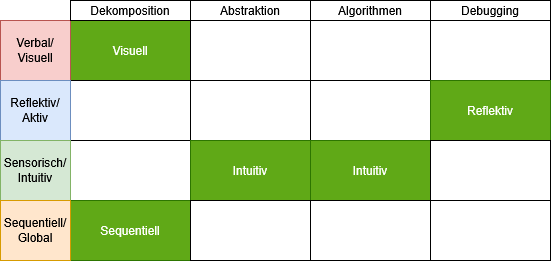
\includegraphics[width=1\linewidth]{Figures/Styles_CT}
    \caption{Vorteile der Lerntypen in den Aspekten des Computational Thinking}
\end{figure}

Für die Computational Thinking Aspekte lässt sich zusammenfassend sagen, dass besonders Personen mit Visuell, Reflektiv, Intuitiv und Sequentiell ausgeprägten Veranlagungen einen Vorteil beim Erlernen der CT Aspekte haben werden.

\begin{figure}[h!]
    \centering
    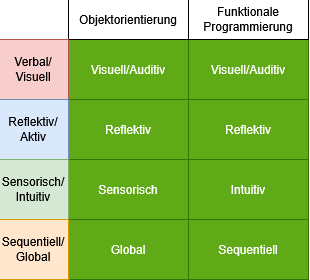
\includegraphics[width=1\linewidth]{Figures/Styles_Paradigms}
    \caption{Vorteile der Lerntypen in den betrachteten Paradigmen}
\end{figure}

Für die Computational Thinking Aspekte lässt sich zusammenfassend sagen, dass besonders Personen mit Reflektiv, Intuitiv und Seuqentiell ausgeprägten Veranlagungen Vorteile beim Lernen mit funktionaler Programmierung haben werden. Personen mit Reflektiv, Sensorischen und Global ausgeprägten Eigenschaften hingegen werden besser mit OO Programmierung lernen.